\section{Abbildungen}
Abbildungen befinden sich in Abbildungsumgebungenen, die
aus mehreren Elementen bestehen. Sie haben:

\begin{itemize}
 \item die Abbildung selbst
 \item eine Unterschrift \lstinline$\caption{}$
 \item ein Label (auf alle(!) Abbildungen muss im Text verwiesen werden)
       \lstinline$\label{}$
\end{itemize}

\begin{lstlisting}
\begin{figure}[h]
 \centering
 \includegraphics[scale=0.02]{HOMO1-Butadien.png}
 \caption{HOMO des Buta-1,3-dien.}
 \label{figure:beispiel}
\end{figure}
\end{lstlisting}

\begin{figure}[h]
 \centering
 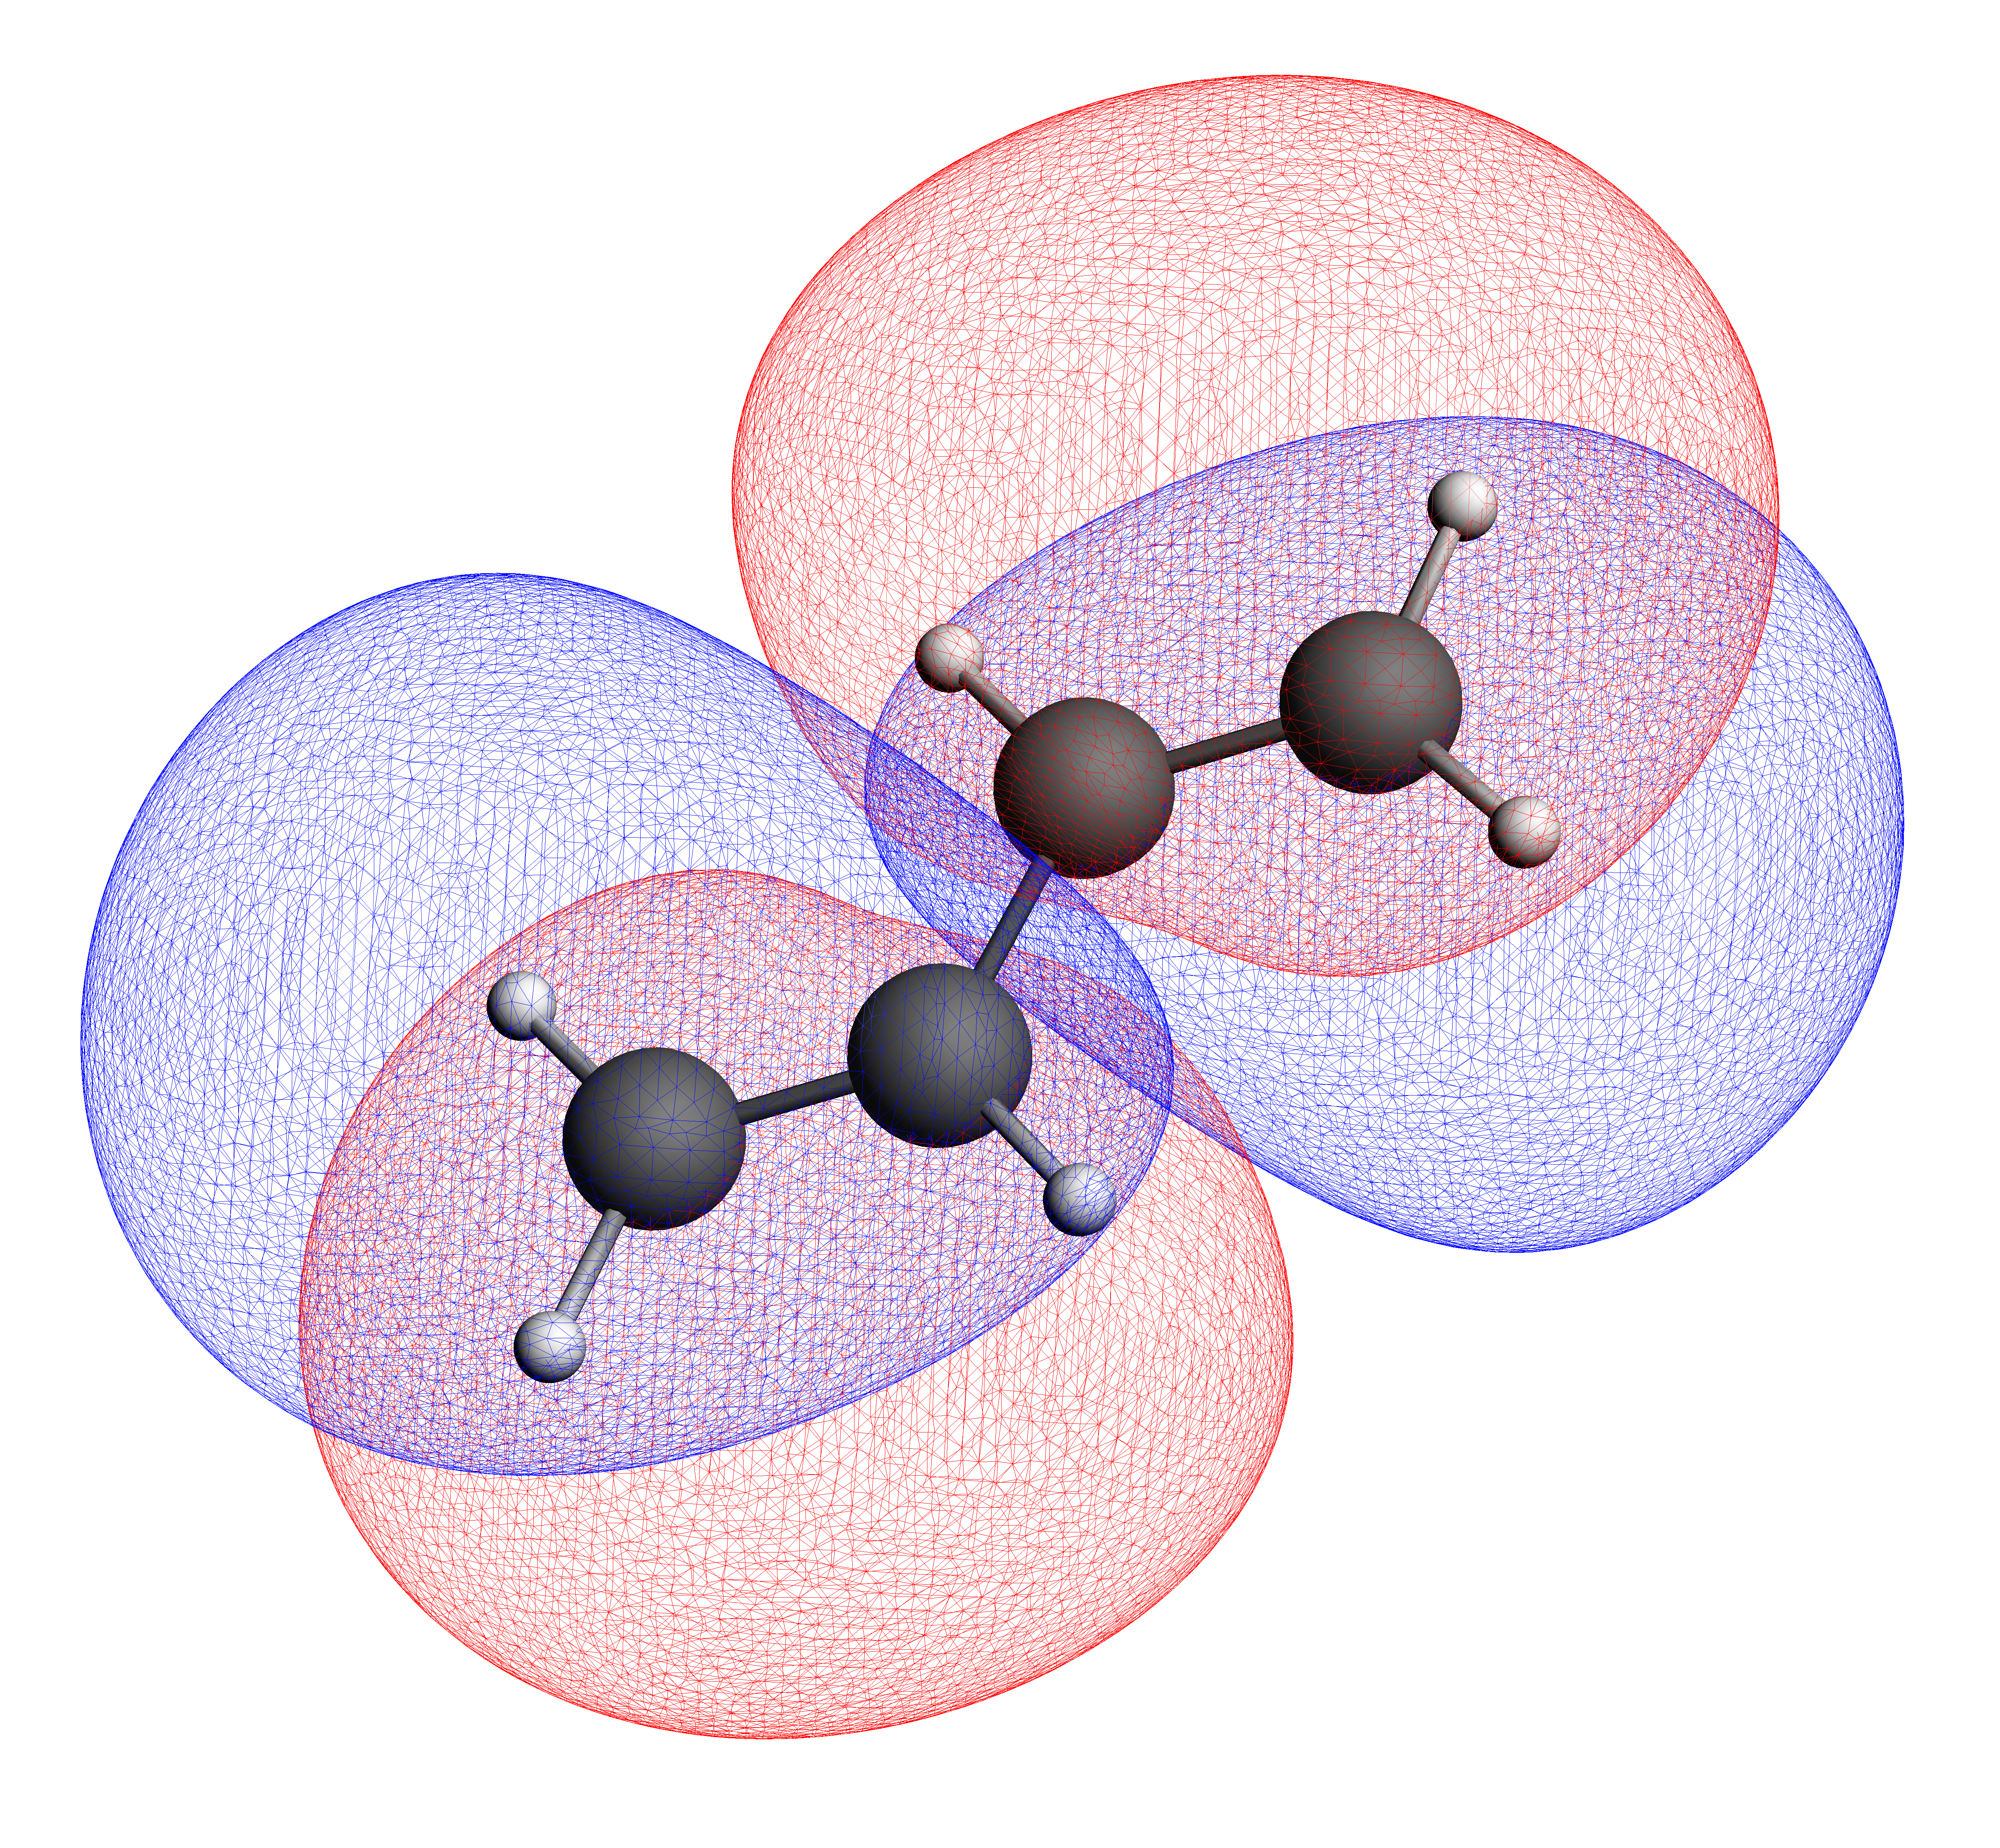
\includegraphics[scale=0.02]{HOMO1-Buten.png}
 \caption{HOMO des Buta-1,2-dien.}
 \label{figure:beispiel}
\end{figure}

\danger Für den Fall der SchülerAkademie muss \lstinline$\figure$ durch
        \textbf{\textbackslash dsafigure} ersetzt werden. Desweiteren ist die
        Option \lstinline$[h]$ im DSA-template nicht zulässig. Sie sollte
        einfach weggelassen werden.
